
\chapter{Introduction}
\label{chapter1}
Reinforcement Learning (RL) \cite{Sutton1998} is based on the idea of learning through experience; it is trial-and-error learning. A decision-making agent learns how to behave in an environment by interacting with it and receiving positive and negative reinforcement. Experience can only be gained by choosing to try new things and observing the consequences; this is known as exploration. However it's often infeasible to try everything, especially in tasks of practical interest, therefore exploration needs to be done in such a way that it gains maximal knowledge about the environment with minimal learning time and costs \cite{Thrun-1992-15850}. However, the agent also needs to utilise its learned knowledge; this is known as exploitation. This gives rise to the so-called \textit{exploration versus exploitation trade-off}; the agent needs to balance exploration and exploitation in such a way that enables both the acquisition and utilisation of knowledge. Consider a human trying to navigate a maze, as in Figure \ref{fig:maze}. Initially, the human has no knowledge about the maze, so they must choose some path to try; if the path they try is realised to lead to a dead end, they might receive some negative reinforcement, and learn that this path is not a good one to take. To escape the maze, the human must try new things; they must explore the maze and discover where the dead ends are, and which paths seem promising, but they also need to exploit the knowledge that they have gained, and follow the promising paths. 
\\Conversely to RL, Automated Planning (or just Planning) \cite{GhallabNauTraverso04, Lav06, DBLP:books/aw/RN2020} uses embedded knowledge of the environment, in the form of a model, to determine the optimal sequence of successive actions to fulfil a given goal. However, planning relies on the model to accurately represent the environment; which cannot be guaranteed, due to approximations, abstractions, and human-error, and therefore planning can be quite fragile. As an example, consider Figure \ref{fig:maze} again. Imagine the human is given a map of the maze, but it shows the true path out of the maze to be a dead end. The human might look at the map and decide it's impossible to escape the maze.
\\Planning and RL take different approaches to decision-making; relying on previously obtained, or embedded, knowledge versus obtaining knowledge through experience. However, they may be combined, which is known as Model-Based RL (MBRL); which is most commonly encapsulated in the form of planning over a learned model, which has been shown to be very effective in recent years \cite{silver2017mastering, pmlr-v28-levine13}. Coming back to the example in Figure \ref{fig:maze}, the human could reason to try the true path that seems like it is a dead end, and realise that it is not actually a dead end, and update the map for the next person.
\\ Exploration is a widely studied topic in RL, since it necessitates learning. Thus, strategies for exploration vary widely. A particularly interesting avenue of research is the use of models within exploration - from using approximate models to constrain exploration, such as DARLING \cite{AIJ16-leonetti}, to using optimistic models to guide exploration, such as OIM \cite{10.1145/1390156.1390288}, to using ensembles of models to derive novel states to explore towards, such as MAX \cite{DBLP:journals/corr/abs-1810-12162}. In practice, however, model-free exploration methods based on randomness, such as $\epsilon$-greedy \cite{conf/nips/Sutton95, Watkins:1989} are ubiquitous.
\\Exploration in RL is still an open problem; many advanced, complex, techniques have been proposed, but the most widely used techniques remain the simplest. Thus, within this work we explore the development of a framework that synergises planning and
learning in order to drive exploration by making intelligent hypotheses about the
environment, informed by the inherently inaccurate, but still useful, model, previous experience
and environmental observations, with the goal being to mitigate model inaccuracies on the quality of learned behaviour, and an overarching aim of distancing the field of exploration from randomness.

% The ultimate goal of this
% work is to mitigate the effect of the inherent inaccuracies in the model on the quality of learned
% behaviour; resulting in agents that can learn beyond the inaccuracies of the model, through
% intelligent exploration.

\begin{figure}[h!]
    \centering
    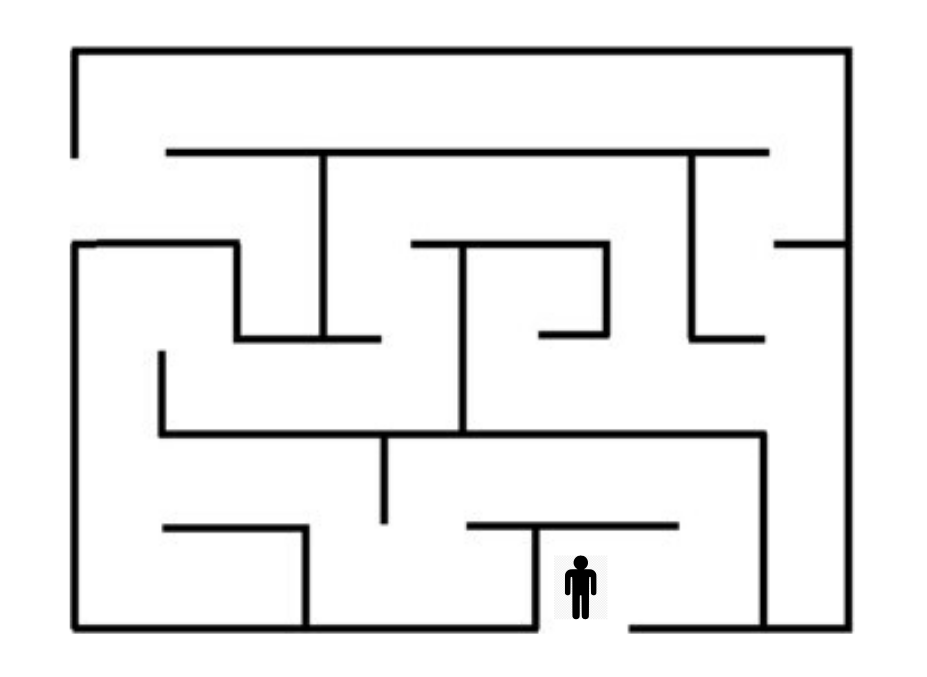
\includegraphics[max size={350pt}{350pt}]{report/assets/maze.png}
    \caption{Maze Navigation}
    \label{fig:maze}
\end{figure}